\documentclass{clbeamer2024}

\usepackage{minted}

\usepackage{minted}
\setminted{
	breaklines=true,
	frame=single,
	bgcolor=lightgray,
	fontsize=\small,
	escapeinside=||
}

\usepackage{xcolor}
\definecolor{bg}{rgb}{0.95, 0.95, 0.92} % Couleur gris clair

\title{
	%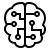
\includegraphics[width=0.5cm]{logos/IA1.png} \hfill
        Introduction aux Cookies
	
\includegraphics[width=0.7cm]{logos/cookie.png} \hfill
}
\subtitle{Comprendre les bases des cookies et leur gestion}
\author{Slimani Mohamed Amine}
\institute{EHTP}
\date{\today}

\begin{document}
	\setcounter{framenumber}{-1}
	\frame{\titlepage}
	
	
	
	% Sommaire
	\begin{frame}{Sommaire}
		\tableofcontents
	\end{frame}
	
	
	\section{Qu'est-ce qu'un cookie ?}
	\begin{frame}{Qu'est-ce qu'un cookie ?}
		\begin{itemize}
			\item \textbf{Définition} : Un cookie est un petit fichier texte stocké sur l'appareil de l'utilisateur par un site web.
			\item \textbf{Objectif} : Enregistrer des informations sur l'utilisateur ou ses préférences.
			\item \textbf{Types de cookies} :
			\begin{itemize}
				\item \textbf{Cookies de session} : Temporaires, supprimés à la fermeture du navigateur.
				\item \textbf{Cookies persistants} : Stockés pendant une durée définie.
			\end{itemize}
		\end{itemize}
	\end{frame}
	
	
	\section{Pourquoi les cookies sont-ils importants ?}
	\begin{frame}{Pourquoi les cookies sont-ils importants ?}
		\begin{itemize}
			\item \textbf{Personnalisation} : Adapter le contenu en fonction des préférences de l'utilisateur.
			\item \textbf{Gestion des sessions} : Maintenir l'état de connexion d'un utilisateur.
			\item \textbf{Analyse} : Suivre le comportement des utilisateurs pour améliorer le site.
		\end{itemize}
	\end{frame}
	
	
	\section{Comment fonctionnent les cookies ?}
	\begin{frame}{Comment fonctionnent les cookies ?}
		\begin{itemize}
			\item \textbf{Création} : Le serveur envoie un cookie au navigateur via l'en-tête HTTP `Set-Cookie`.
			\item \textbf{Stockage} : Le navigateur stocke le cookie localement.
			\item \textbf{Envoi} : Le navigateur renvoie le cookie au serveur à chaque requête via l'en-tête HTTP `Cookie`.
		\end{itemize}
	\end{frame}
	
	\begin{frame}{Schéma Explicatif }
		\begin{center}
		    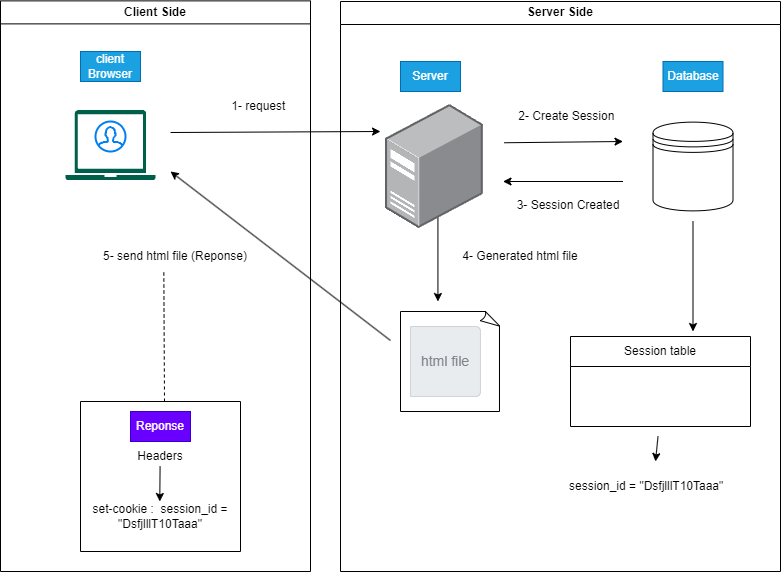
\includegraphics[width=10cm]{test/schema.png} 
		\end{center}
		
		 
			
	\end{frame}
	
	\section{Types de cookies}
	\begin{frame}{Types de cookies}
		\begin{itemize}
			\item \textbf{Cookies essentiels} : Nécessaires au fonctionnement du site (ex : gestion des sessions).
			\item \textbf{Cookies de préférence} : Enregistrent les choix de l'utilisateur (ex : langue, thème).
			\item \textbf{Cookies analytiques} : Collectent des données pour l'analyse du trafic.
			\item \textbf{Cookies de publicité} : Suivent les utilisateurs pour afficher des publicités ciblées.
		\end{itemize}
	\end{frame}


\section{Sécurité et confidentialité}
\begin{frame}{Sécurité et confidentialité}
	\begin{itemize}
		\item \textbf{Risques} : Vol de cookies, suivi non consenti.
		\item \textbf{Protection} : Utiliser des cookies sécurisés (flag `Secure`), limiter la durée de vie des cookies.
		\item \textbf{Régulations} : RGPD (UE), CCPA (Californie) exigent le consentement des utilisateurs.
	\end{itemize}
\end{frame}


\section{Exemple de gestion des cookies en JavaScript}
\begin{frame}{Exemple de gestion des cookies en JavaScript}
	\begin{exampleblock}{Code JavaScript}
			\begin{center}
			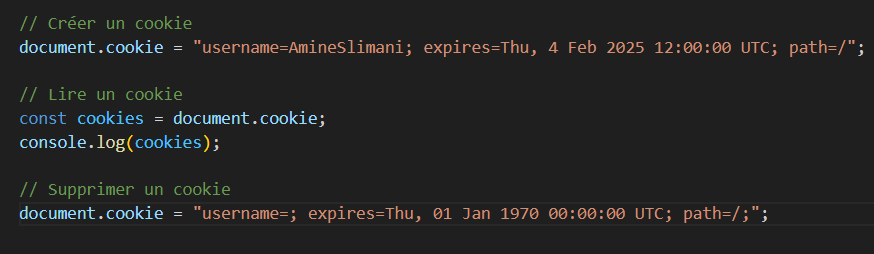
\includegraphics[width=10cm]{test/code.png} 
		\end{center}
		
	\end{exampleblock}
\end{frame}

\section{Bonnes pratiques}
\begin{frame}{Bonnes pratiques}
	\begin{itemize}
		\item \textbf{Minimiser les données} : Ne stocker que les informations nécessaires.
		\item \textbf{Sécuriser les cookies} : Utiliser les flags `Secure` et `HttpOnly`.
		\item \textbf{Obtenir le consentement} : Informer les utilisateurs et obtenir leur accord.
	\end{itemize}
\end{frame}

\section{Outils pour gérer les cookies}
\begin{frame}{Outils pour gérer les cookies}
	\begin{itemize}
		\item \textbf{Google Analytics} : Suivi des utilisateurs et analyse du trafic.
		\item \textbf{Cookiebot} : Gestion du consentement des cookies conformément au RGPD.
		\item \textbf{Browser Developer Tools} : Inspecter et gérer les cookies dans le navigateur.
	\end{itemize}
\end{frame}


\section{Exemple de politique de cookies}
\begin{frame}{Exemple de politique de cookies}
	\begin{itemize}
		\item \textbf{Objectif} : Informer les utilisateurs sur l'utilisation des cookies.
		\item \textbf{Contenu} :
		\begin{itemize}
			\item Types de cookies utilisés.
			\item Objectif de chaque cookie.
			\item Comment refuser ou gérer les cookies.
		\end{itemize}
	\end{itemize}
\end{frame}

\section{Pourquoi c'est important ?}
\begin{frame}{Pourquoi c'est important ?}
	\begin{itemize}
		\item Les cookies sont essentiels pour personnaliser l'expérience utilisateur et gérer les sessions.
		\item Ils soulèvent des questions de confidentialité et de sécurité.
		\item Comprendre les cookies est crucial pour les développeurs web et les professionnels du numérique.
	\end{itemize}
\end{frame}

\begin{frame}{Résumé}
	\textbf{Les cookies} sont des outils essentiels pour personnaliser l'expérience utilisateur et gérer les sessions, mais ils nécessitent une gestion responsable pour garantir la confidentialité et la sécurité.
\end{frame}



	
	
\end{document}
